\documentclass[12pt]{article}
\usepackage[hidelinks]{hyperref}    
\usepackage[all]{hypcap}
\usepackage{graphicx}
\graphicspath{{../images/}} % imposta path per trovare le immagini, i .. significano "la dir precedente"
\author{Andrea Malvezzi}
\title{\textbf{Architettura degli Elaboratori~-~Porte logiche e circuiti combinatori}}  % textbf = testo bold
\date{26 Settembre, 2024}
\author{Andrea Malvezzi}
\begin{document}
\maketitle
\pagebreak
\tableofcontents
\pagebreak
\section{Algebra di Boole}
\subsection{Espressioni booleane}
Un'espressione booleana si costruisce usando:
\begin{itemize}
    \item 0 e 1 (False e True);
    \item gli operatori booleani (o logici);
    \item delle variabili sempre con valore 0 oppure 1.
\end{itemize}
\subsection{Proprietà dell'algebra di Boole}
Nella tabella seguente sono presenti delle equivalenze per descrivere le proprietà dell'algebra di Boole.
\begin{figure}[!htb]
    \centering
    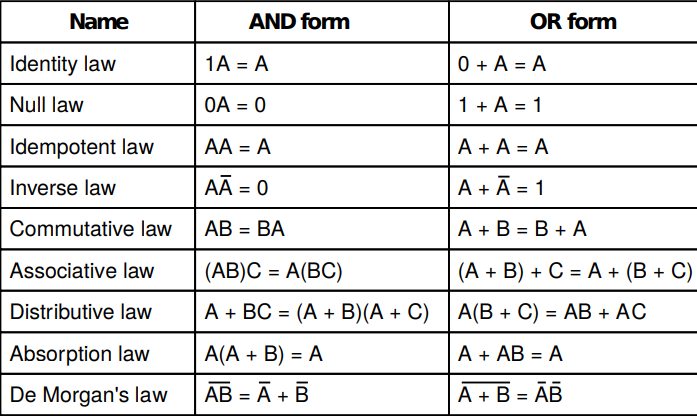
\includegraphics[width=1\textwidth, height=.7\textheight,keepaspectratio]{porte_logiche/properties_boole.png} % essenzialmente resiza l'immagine
    \begin{center}
        \caption{\label{fig:properties_boolean_algebra}Una visualizzazione delle proprietà dell'algebra di Boole.} % label fuori da caption spesso non va, mettilo dentro
    \end{center}
\end{figure}
\pagebreak
\subsubsection{La legge di De Morgan}
La più importante tra le leggi presentate è sicuramente quella di De Morgan,\\
in quanto permette di passare da una colonna della tabella all'altra in modo semplice e veloce.
\subsubsection{Esempio di applicazione della legge di De Morgan}
\begin{itemize}
    \item Per cominciare, scriviamo la OR form della legge inversa: $A + \overline{A} = 1$;
    \item Seguentemente occorre pensare a com'è scritta l'espressione: siamo\\davanti ad una OR tra due variabili A, di cui una negata, il tutto pari ad 1;
    \item Ora osserviamo la legge di De Morgan nella forma OR. Questa afferma quanto segue: La negazione di una OR equivale ad una AND con entrambi gli input negati;
    \item Applichiamo quindi De Morgan: $\overline{A} + A = 1$ diventerà $\overline{A\overline{A}} = \overline{1}$, ovvero $\overline{A}A = 0$.
\end{itemize}
Ed ecco mostrato come passare da un lato all'altro della tabella tramite la formula di De Morgan.
\subsection{Formula canonica}
Una funzione booleana si può definire attraverso un'espressione basata solamente sulla AND, la OR e la NOT.\\
Inoltre, una funzione booleana è esprimibile in una forma detta "canonica". Per ricavarla occorre:
\begin{itemize}
    \item identificare tutte le combinazioni per cui la funzione in esame è vera (queste son dette \textbf{mintermini});
    \item fare la OR dei mintermini trovati;
\end{itemize}
\pagebreak
\subsubsection{Esempio di formula canonica}
Analizziamo la seguente tabella:
\begin{figure}[!htb]
    \centering
    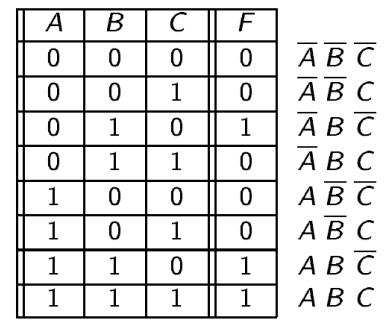
\includegraphics[width=.7\textwidth, height=.7\textheight,keepaspectratio]{porte_logiche/canonica.png} % essenzialmente resiza l'immagine
    \begin{center}
        \caption{\label{fig:canonica_esempio}Nella tabella presentata si hanno 3 mintermini: $\overline{A}B\overline{C}$, $AB\overline{C}$, $ABC$.} % label fuori da caption spesso non va, mettilo dentro
    \end{center}
\end{figure}\\
Ora dobbiamo fare la OR tra i 3 mintermini trovati precedentemente:
\begin{center}
    $\overline{A}B\overline{C} + AB\overline{C} + ABC$
\end{center}
Questa espressione equivale alla forma canonica della funzione studiata.
\pagebreak
\section{I transistor}
Un transistor è un dispositivo a 3 connettori: \textbf{collettore}, \textbf{emettitore} e \textbf{base}.\\
Quando non c'è tensione sulla base, il componente agisce come una resistenza infinita tra emettitore e collettore.\\
In caso contrario, si comporta da conduttore ideale.
\begin{figure}[!htb]
    \centering
    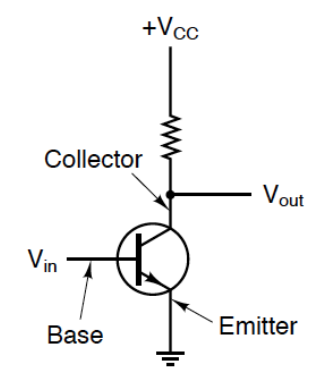
\includegraphics[width=.7\textwidth, height=.7\textheight,keepaspectratio]{porte_logiche/transistor_not_ex.png} % essenzialmente resiza l'immagine
    \begin{center}
        \caption{\label{fig:transistor_not_esempio}Esempio di porta NOT realizzata con transistor.} % label fuori da caption spesso non va, mettilo dentro
    \end{center}
\end{figure}
\subsection{La porta NOT realizzata tramite transistor}
La porta NOT della figura (\ref{fig:transistor_not_esempio}) funziona nella seguente maniera:
\begin{itemize}
    \item quando l'ingresso \textit{V\textsubscript{in}} è \textit{alto}, la corrente \textit{V\textsubscript{cc}} attraversa il transistor e lascia \textit{V\textsubscript{out}} basso (Input 1, output 0);
    \item quando l'ingresso \textit{V\textsubscript{in}} è \textit{basso}, la corrente \textit{V\textsubscript{cc}} non riesce ad attraversare il transistor, il quale agisce da resistenza infinita, passando quindi per \textit{V\textsubscript{out}}, il quale diventa alto (Input 0, output 1).
\end{itemize}
\subsection{La porta NAND realizzata tramite transistor}
\end{document}